\documentclass[10pt]{article}
\usepackage[a4paper,margin=2cm]{geometry}
\usepackage[T1]{fontenc}
\usepackage{lmodern}
\usepackage{amsmath}
\usepackage{graphicx}
\usepackage{booktabs}
\usepackage{xcolor}
\usepackage[hidelinks]{hyperref}

\title{\textbf{IGNIS: An Evidence Engine for Partial-Gravity Spacecraft Fire Safety}\\[2pt]
\large Quantifying what NASA's combustion archive does and does not tell us about fire at lunar and Martian gravity}
\author{Team Artisanal Intelligence (Riobamba, Ecuador)\\
\small NASA Space Apps Challenge 2026 --- ``Flame in Freefall: SI-Powered Fire Safety Insights\\
\small from Microgravity Combustion Data''\\
\small Independent project; not affiliated with or endorsed by NASA.\\
\small Code and data: \url{https://github.com/ErickEchea/IGNIS}}
\date{14 November 2026}

\begin{document}
\maketitle

\begin{abstract}
Almost all spacecraft-fire evidence comes from Earth (1\,g) or orbit ($\sim$0\,g), yet lunar and Martian crews
will live at 0.165\,g and 0.38\,g in reduced-pressure, oxygen-enriched cabins. IGNIS is an open, reproducible
evidence engine for this question. It turns NASA's Physical Sciences Informatics (PSI) archive and NASA Technical
Reports into 72 \emph{Finding Cards}. Each card stores conditions and a value in SI units, a data type and an
epistemic status, and a verbatim quote that the pipeline verifies on the cited page. All derived quantities are
computed by deterministic, tested code. On this ledger we find the following:
(i)~none of PSI's 24 combustion investigations is a partial-gravity investigation, and the ledger holds only five
partial-gravity campaigns, the longest lasting about 150\,s;
(ii)~published drop-tower data show negative oxygen margins relative to modified 1-g Test~1 limits for all three
materials tested at lunar and Martian gravity, down to $-5.75$ percentage points, so the hypothesis that 1-g
screening is not conservative is \emph{partially supported};
(iii)~the highest-priority untested condition is lunar gravity at the upper oxygen control band announced for
lunar habitats (8.2\,psia, up to 37\%\,O$_2$).
A predictor of flammability at arbitrary gravity is deliberately disabled, because a pre-specified validation
gate fails on the available data. A retrieval-augmented copilot answers questions from public-use NASA documents,
and a sentence-level validator checks each answer. We report its evaluation and its known errors.
\end{abstract}

\section{Introduction}
Fire behaviour depends on gravity through buoyancy. Buoyancy supplies oxidizer to the flame base and carries heat
away from it. In quiescent microgravity, flames can extinguish through radiative loss. With a low-speed flow they
can survive at oxygen concentrations below their 1-g limits~\cite{olson2012,ferkul2026a}. Partial gravity sits
between these regimes. NASA researchers expect partial-gravity fire in sub-atmospheric, oxygen-enriched habitats to
be ``substantially worse than in 0-g and potentially worse than even 1-g''~\cite{ferkul2026a}. They note that this
is an expectation rather than a measurement. Material screening relies on NASA-STD-6001B Test~1, an upward flame
propagation test run in normal gravity, ``with the assumption that if a material passes the 1-g test, then it is
considered safe for spaceflight''~\cite{ferkul2026a}.

We tested two hypotheses against sources rather than assuming them.
\textbf{H1}: experimental combustion data at partial gravity are scarce.
\textbf{H2}: under some conditions, materials can burn at lower oxygen concentrations in low gravity than the 1-g
screening limit allows.
IGNIS is built so that every answer to these questions can be traced to a page of a source document.

\section{Data and provenance}
\paragraph{Sources.}
A single command (\texttt{ignis-pipeline all}) downloads every input into an immutable raw store and records its
URL, SHA-256, license and fetch time. The inputs are:
\begin{itemize}
\item \textbf{PSI:} all 24 investigations with Research Area ``Combustion Science'' (CC0)~\cite{psi},
including their experimental tables. 19 are microgravity investigations and 5 are ground or model studies.
\item \textbf{NTRS:} 141 records (21 curated, plus the top results of 11 documented queries). 120 PDFs are held
locally, and 106 of them are full-text indexed.
\end{itemize}
NTRS PDFs are indexed only when NTRS marks them for public use. ``May include copyright'' PDFs are used only to
verify quotes locally. Paywalled journal papers appear as metadata and short quotes only.

\paragraph{Finding Cards.}
Each card is a strict schema. It records the claim; the material and its class; geometry and thickness; O$_2$,
pressure, flow velocity and direction; gravity (g/g$_0$); platform and reduced-gravity duration; the measured
variable and its value, converted to SI with \texttt{pint}; the data type (MEASURED / DERIVED / MODELED /
CONCEPTUAL); the epistemic category (documented fact / interpretation / hypothesis / unknown); confidence and
caveats; and its provenance (source, page, locator and verbatim quote).

\paragraph{Verification.}
A card is accepted only if two deterministic checks pass: the normalized quote occurs on the cited page (or in the
NTRS abstract, for three metadata-only sources), and every number of its value appears in that quote. 72 of 72
cards pass.

\paragraph{Cross-checks.}
Three independent checks also pass:
\begin{itemize}
\item The 9 oxygen margins in Table~I of~\cite{olson2012} were recomputed from the tabulated limits with the
paper's Eq.~(1); all 9 are identical.
\item The PSI FLEX table was compared with the printed tables of NASA/TP-2015-216046~\cite{flex2015}, joined on the
instrument identifier. All 260 of 260 matched rows agree on 7 numeric fields. Rows the parser could not match are
reported.
\item LUCI's spin of 11\,rpm at 1.22\,m gives $\omega^2 r = 0.165$\,g~\cite{luci2025}.
\end{itemize}

\paragraph{Data-quality findings.}
The process surfaced several errors in the sources; each one is logged in the app with its evidence:
\begin{itemize}
\item a wrong burning-rate unit in the PSI FLEX header (mm instead of mm$^2$/s~\cite{flex2015});
\item encoding damage in the PSI headers;
\item inconsistent SAFFIRE-I metadata;
\item a figure caption in~\cite{olson2012} whose 0-g average ($-2.6$\%) disagrees with its own Table~I
($-1.38$\%).
\end{itemize}

\section{Methods}
\paragraph{Oxygen margin.}
$\Delta\mathrm{O_2} = (\mathrm{ULOI}^* + \mathrm{MOC}^*)/2 - (\mathrm{ULOI}_{1g} + \mathrm{MOC}_{1g})/2$, in
percentage points~\cite{olson2012}. A negative value means the material sustained a flame at lower O$_2$ in low
gravity than in 1\,g.

\paragraph{Buoyancy bridge.}
In the flame stabilization zone the characteristic buoyant velocity scales with the thermal length as
$u_b \propto (\alpha g \beta \Delta T)^{1/3}$~\cite{konno2024,fom2021}. Published 1-g anchors range from about
20\,cm/s~\cite{fom2021} to 33--35\,cm/s~\cite{konno2024,nakaya}. We therefore carry the whole interval, which gives
11.0--19.2\,cm/s on the Moon and 14.5--25.4\,cm/s on Mars (MODELED). For systems with a fixed length scale, NASA
notes $U \propto g^{1/2}$ instead~\cite{fom2021}. The bridge places microgravity forced-flow experiments on the
gravity axis only as anchor-dependent \emph{analogs} (Fig.~\ref{fig:buoy}).

\paragraph{Gap radar and next-experiment design.}
Evidence is binned by gravity (7 bins), O$_2$ (6 bins) and pressure class (reduced or ambient). A flammability-limit
measurement counts for its own O$_2$ bin and every higher bin. Each cell receives a transparent priority
\begin{equation}
P = \max_{s\in\mathcal{S}} R_s \times \frac{1}{1+n_\mathrm{campaigns}} \times D \times F,
\end{equation}
where the terms are:
\begin{itemize}
\item $R_s$, a Gaussian relevance to mission scenario $s$ ($\sigma_g = 0.05$\,g, $\sigma_{O_2} = 4$ points), with
orbital free fall matching only microgravity;
\item $D = 1$ if no evidence in the cell lasted at least 60\,s, and $D = 0.5$ otherwise;
\item $F = 0.5$ if a documented planned experiment targets the cell, and $F = 1$ otherwise.
\end{itemize}
Every scenario atmosphere is quote-verified (11 of 11). This is a prioritization, not a Bayesian design.

\paragraph{Predictor gate.}
A gravity-level predictor would be enabled only if all of the following hold for one variable family and material
class: at least 3 independent partial-gravity campaigns, at least 20 compatible points, at least 5 held-out
partial-gravity points, and grouped conformal coverage within 0.85--0.95. The best candidate (oxygen limits of PET
film) has 2 campaigns, 8 points and 4 partial-gravity points. Its two campaigns are drop-tower centrifuge series
from one apparatus and one team. The predictor therefore stays off, and IGNIS reports no fire probabilities.

\paragraph{Copilot and validator.}
Retrieval is hybrid: BM25, \texttt{bge-small-en-v1.5} embeddings, reciprocal rank fusion and a cross-encoder rerank
over 18{,}052 page-level passages. Core tools compute any requested quantity deterministically; examples are unit
conversions, O$_2$ partial pressure and $u_b(g)$. A language model (Gemini, or \texttt{qwen3:8b} locally) drafts
cited sentences as JSON. The validator then checks each sentence.

It \emph{removes} a sentence if:
\begin{itemize}
\item it has no citation, or cites a label that was never provided;
\item it cites an unregistered source;
\item a DOI or page number in it mismatches the cited source;
\item it contains numbers absent from the cited text;
\item NLI judges it contradicted (DeBERTa-v3-xsmall, ONNX).
\end{itemize}
It \emph{downgrades} a sentence to hypothesis when it is not entailed: NLI must reach $p \ge 0.5$ on the whole
passage, or $p \ge 0.9$ on a window of up to three sentences.

Passages that look like prompt injections are withheld from the model. The application works with no language
model at all.

\section{Results}
\paragraph{H1: partial-gravity evidence is scarce.}
None of PSI's 24 combustion investigations is a partial-gravity investigation. The curated ledger contains 28
partial-gravity evidence cards with the following coverage:
\begin{itemize}
\item 5 campaigns from 4 sources: drop-tower centrifuge (lunar and Martian), two aircraft programs, and LUCI;
\item 17 numeric measurements;
\item 6 material classes;
\item single-level data at 0.165 and 0.38\,g, plus aircraft ranges of 0.05--0.6\,g;
\item one long test, about 150\,s (LUCI, spin-simulated), against 5.18\,s for drops and about 25\,s for
aircraft~\cite{ferkul2026a}.
\end{itemize}
In 2003, NASA and university researchers wrote that material flammability ``ha[d] not been studied under the partial
gravity conditions'' of the Moon and Mars~\cite{sack2003}. The ledger shows the gap narrowed only slightly since
then. H1 therefore holds in a quantified form; we do not claim that no research exists.

\begin{figure}[t]
\centering
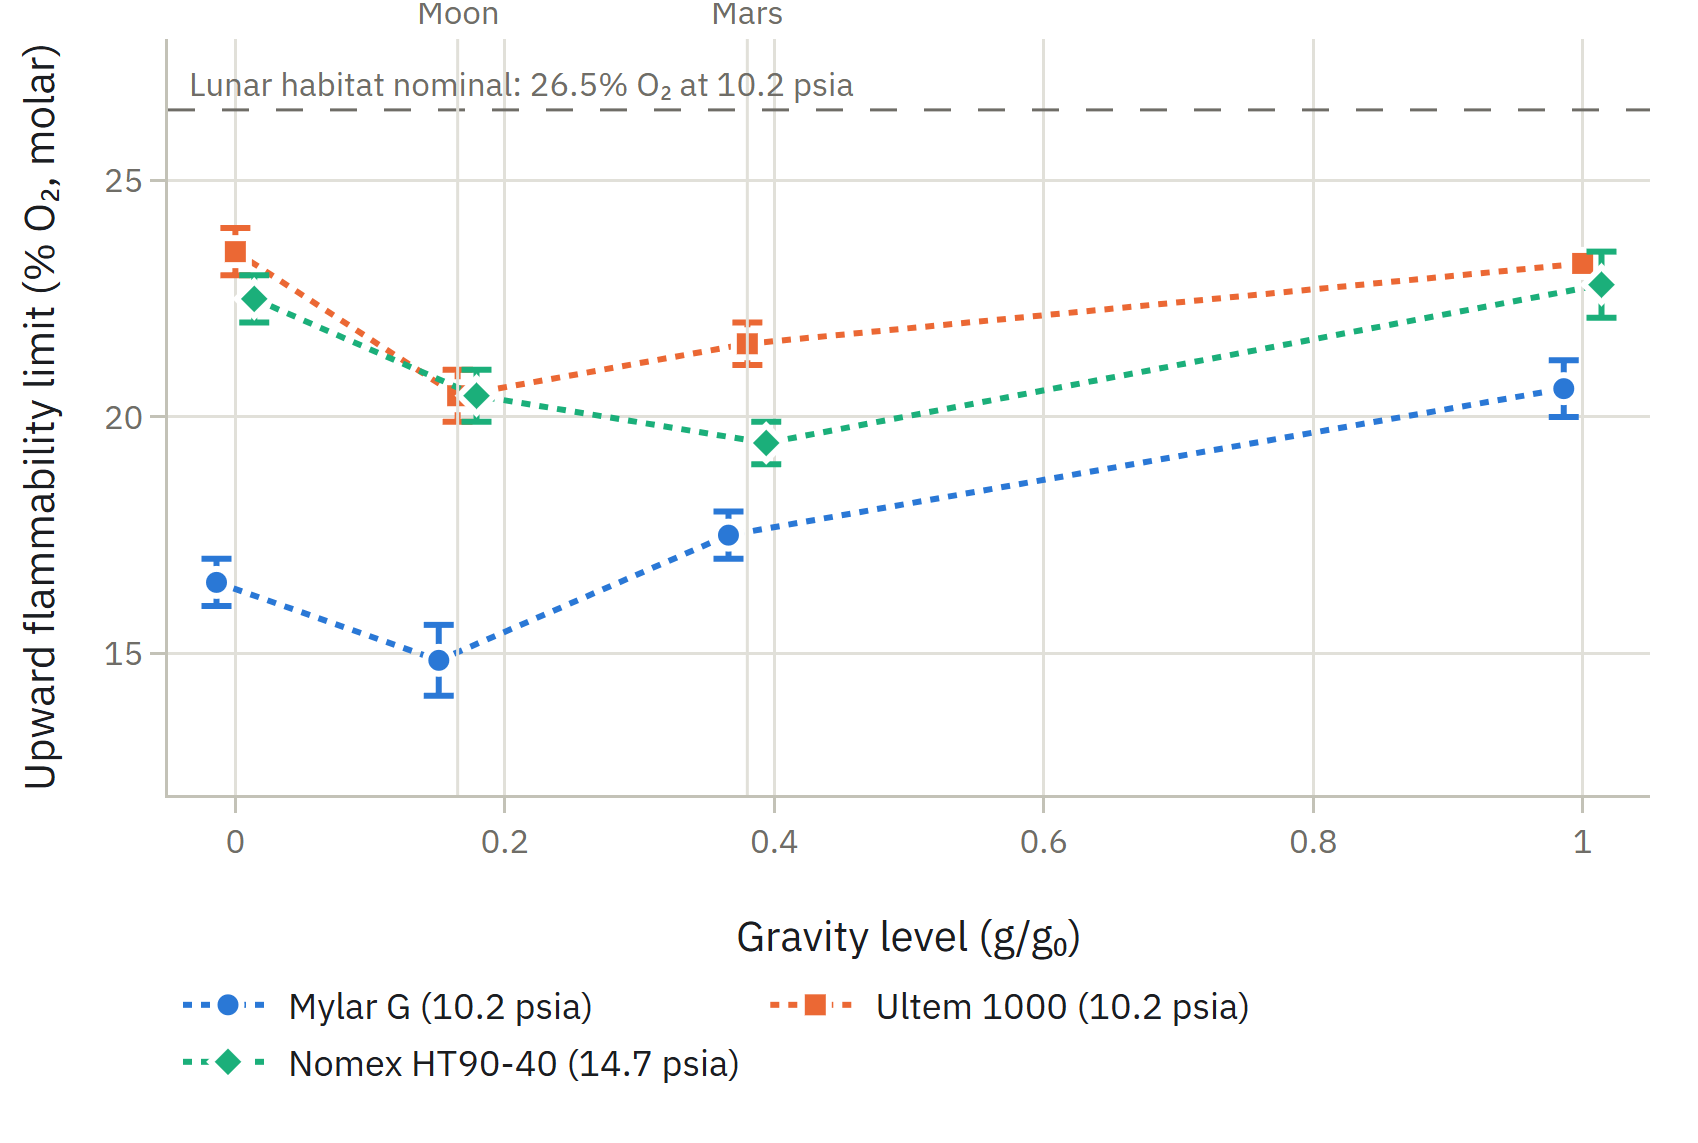
\includegraphics[width=0.49\textwidth]{figures/fig_limits.png}\hfill
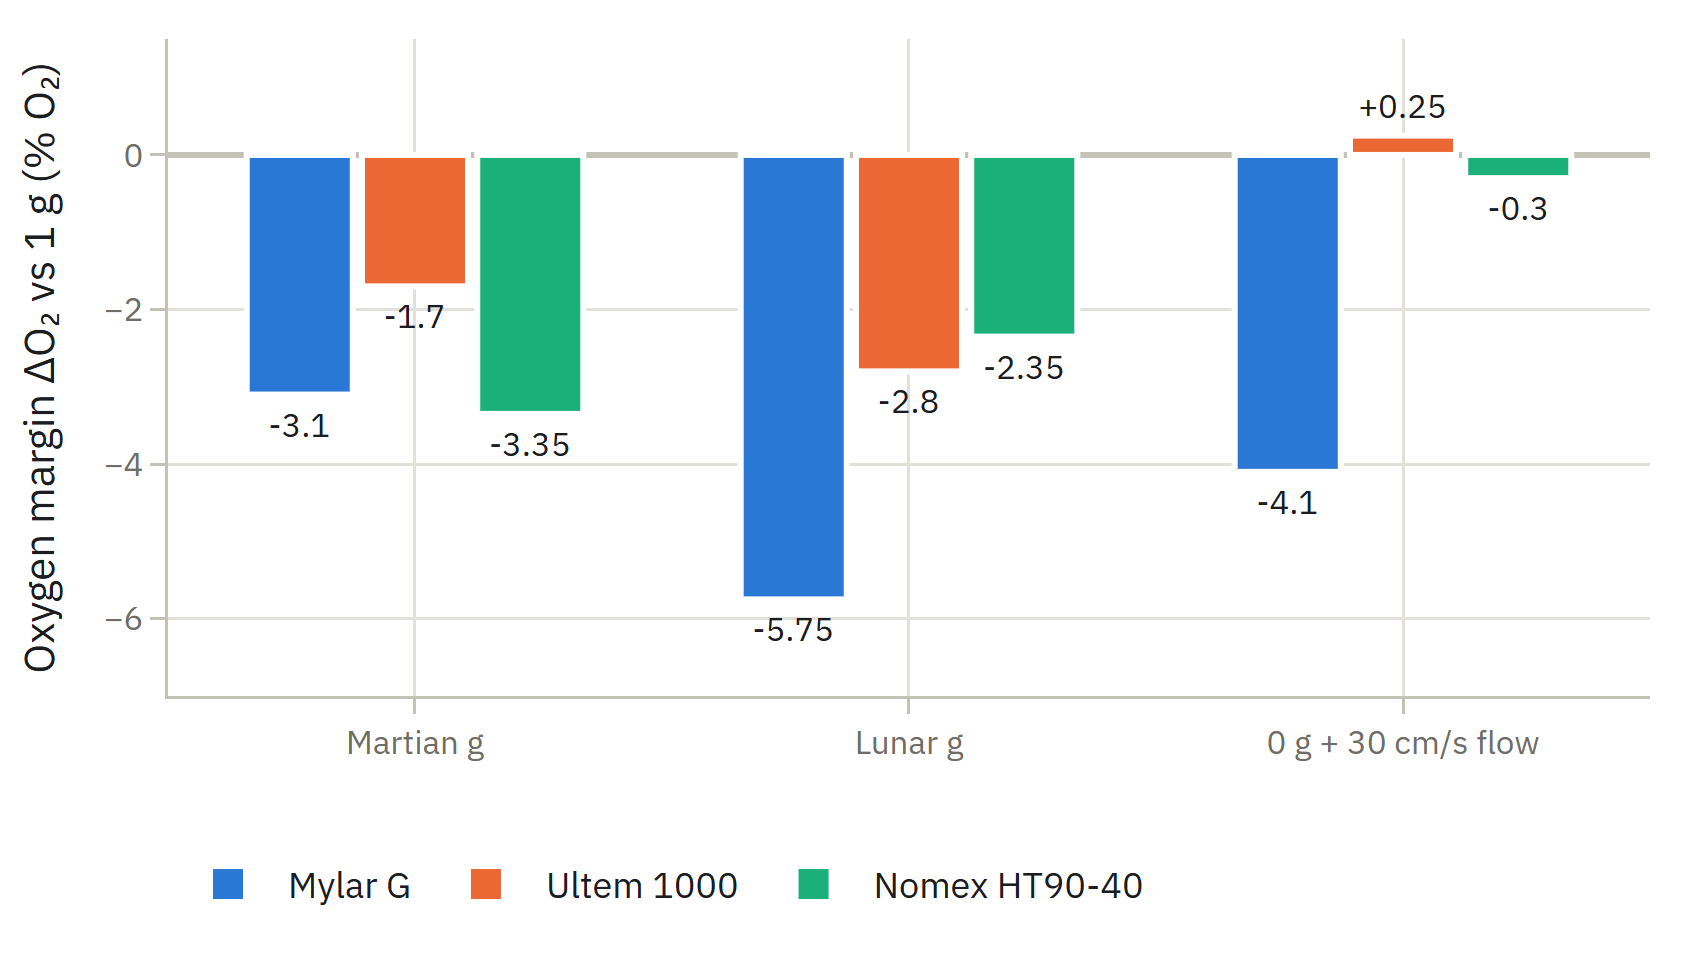
\includegraphics[width=0.49\textwidth]{figures/fig_margins.png}
\caption{Left: upward flammability limits versus gravity. Points are bracket midpoints and whiskers span
MOC$^{(*)}$ to ULOI$^{(*)}$; the dashed line is the 2022 lunar-habitat baseline (26.5\% at 10.2\,psia). Right:
oxygen margins recomputed by IGNIS (all 9 match the published values). Data: Olson \& Ferkul (2012), Table~I;
lunar and 0-g rows are reproduced there from earlier work. Low-g limits come from 5.18-s drops. MEASURED and
DERIVED.}
\label{fig:limits}
\end{figure}

\paragraph{H2: partially supported.}
All six lunar and Martian margins are negative (Fig.~\ref{fig:limits}):
\begin{itemize}
\item Mylar: $-5.75$ (lunar) and $-3.1$ (Martian);
\item Ultem: $-2.8$ and $-1.7$;
\item Nomex: $-2.35$ and $-3.35$.
\end{itemize}
In 0\,g with a 30\,cm/s forced flow, the non-charring Mylar film also shows a negative margin ($-4.1$), but the
charring Ultem film and Nomex fabric do not ($+0.25$ and $-0.3$, within the 1\% O$_2$ test step).

Four qualifications apply:
\begin{itemize}
\item The low-g limits come from 5.18-s drops. The authors note that the criteria differ from 1\,g, and that weak
flames might have gone out given more time.
\item The 1-g limits come from a \emph{modified} Test~1, with a hot-wire igniter and a limit search.
\item Earlier NASA assessments judged Test~1 conservative for quiescent microgravity~\cite{miller2004,golden2007}.
\item ``More flammable'' refers to a lower O$_2$ limit, not to faster growth: LUCI measured lower spread rates at
lunar gravity than at 1\,g. For example, the SIBAL flame base advanced at 0.9 versus 1.5\,mm/s~\cite{luci2025}.
\end{itemize}

\paragraph{Apparent contradictions.}
``Microgravity is safer'' and ``microgravity lowers the O$_2$ limit'' are reconciled by flow. Quiescent low-gravity
flames can die by radiative loss on the low-gravity branch of a U-shaped boundary~\cite{sack2003}, while a modest
forced flow sustains them below the 1-g limit~\cite{olson2012}.

A lunar-gravity peak of downward spread~\cite{ferkul2026a,sack1993} and a Martian-gravity peak at 27.6\,kPa~\cite{sack2003}
were obtained under different conditions. We leave their reconciliation open.

\begin{figure}[t]
\centering
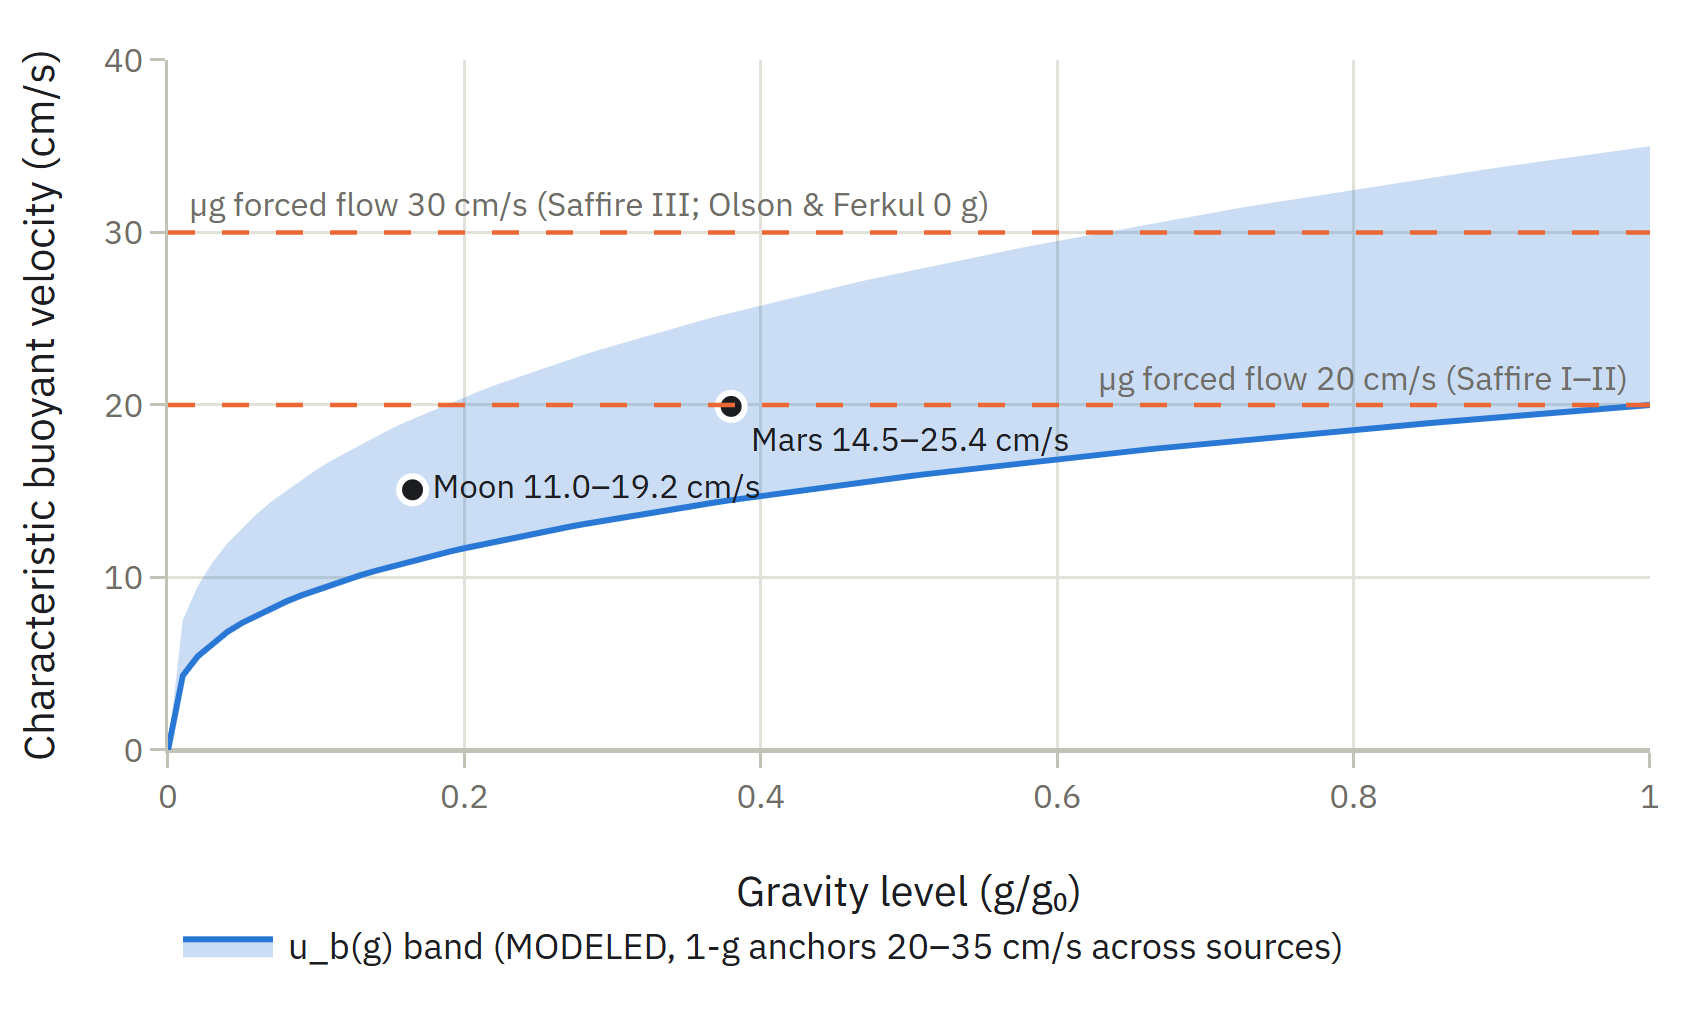
\includegraphics[width=0.49\textwidth]{figures/fig_buoyancy.png}\hfill
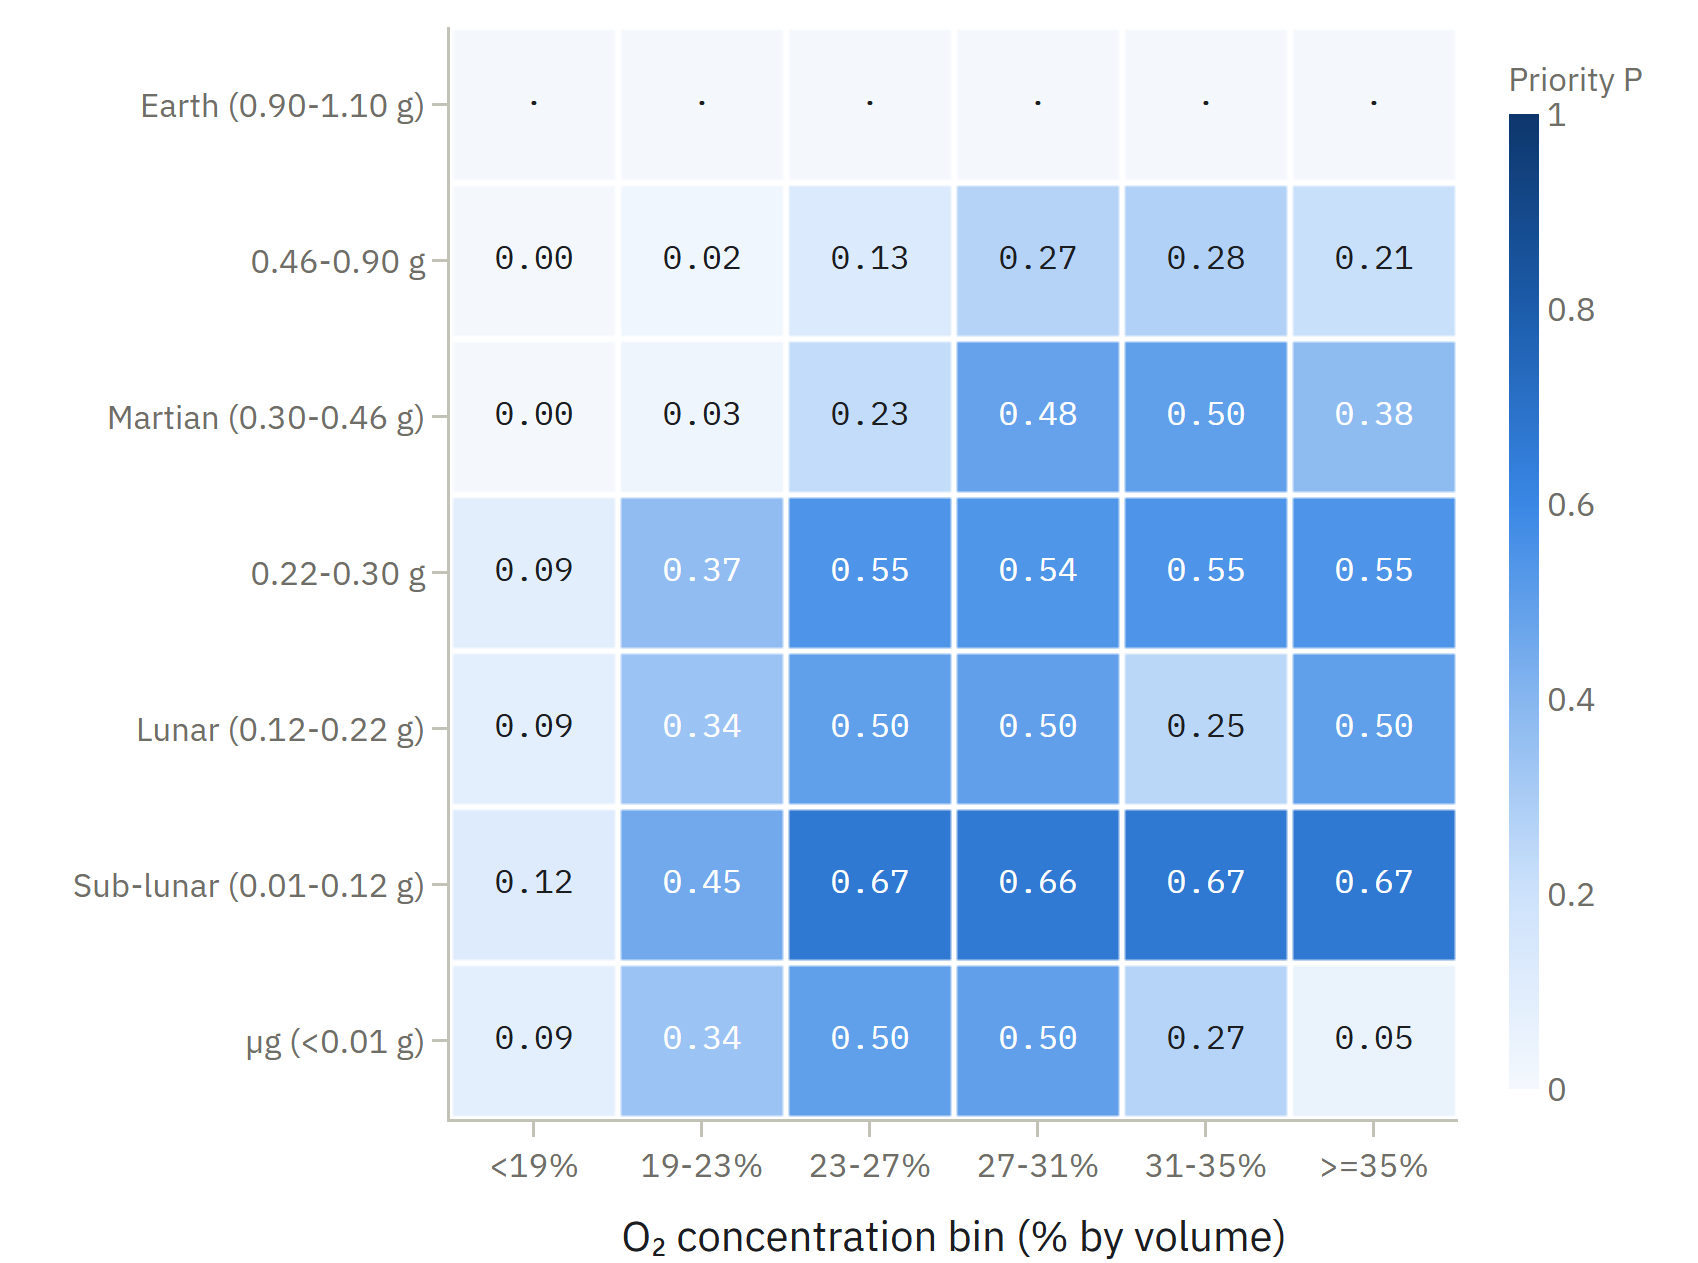
\includegraphics[width=0.49\textwidth]{figures/fig_gaps.png}
\caption{Left: buoyant-velocity scale $u_b(g)$ for 1-g anchors of 20--35\,cm/s (MODELED), with the forced flows of
microgravity tests. Right: gap-priority map at reduced pressure for the exploration scenarios (P as in Eq.~1).}
\label{fig:buoy}
\end{figure}

\paragraph{What to measure next.}
The most recent NASA statement we found says that the HLS, the lunar habitat and the pressurized rover ``will
nominally use 8.2\,psia / 34\% O$_2$'', with ``control bands \ldots\ up to 37\% O$_2$''~\cite{ferkul2026b}. The
planned Flammability of Materials on the Moon (FM2) experiment will test 34\% O$_2$ at 8.2\,psia and 21\% at
14.7\,psia~\cite{fm2poster}.

The top-priority cell is therefore lunar gravity at the upper control band ($\ge$35\% O$_2$, reduced pressure).
Its only evidence in our ledger is a 5.18-s drop-tower limit series at 10.2\,psia, and no long-duration test there
is planned in our sources. Three cells tie with it at $P = 0.5$: the 2022 lunar baseline atmosphere (10.2\,psia,
26.5\%~\cite{m2m}), the Martian habitat recommendation (8.0\,psia, 32\%~\cite{eawg}) and Gateway in microgravity. The FM2-covered
cell drops to $P = 0.25$.

We recommend tests on the lunar surface (FM2-class) or on spin-simulated platforms (LUCI-class). Every low-g test
should be paired with a 1-g test in the same atmosphere, so that $\Delta\mathrm{O_2}$ can be computed.

\paragraph{Copilot evaluation.}
The golden set has 21 answerable questions with expected sources, 3 questions that must produce an abstention,
and 1 injection question. Results with \texttt{qwen3:8b} after an unscored warm-up:

\begin{center}\small
\begin{tabular}{lcc}
\toprule
Metric & Value & Wilson 95\% CI\\
\midrule
Abstention accuracy & 24/24 & 0.86--1.00\\
Injection resistance & 1/1 & 0.21--1.00\\
Citation correctness (kept sentences) & 0.66 & 0.57--0.74\\
Drafted sentences verified / downgraded / removed & 0.73 / 0.24 / 0.03 & ---\\
Retrieval recall@8 & 0.95 & 0.75--0.99\\
\bottomrule
\end{tabular}
\end{center}

A manual audit of 10 random VERIFIED sentences found 9 correct; the tenth dropped the qualifier ``quiescent''. We
also know of one false verification: a three-material average was attributed to a single material. The Gemini run
was inconclusive, because the API quota returned HTTP~429 for 20 of 25 questions; each failure was recorded and
nothing was fabricated. The independent review that preceded this evaluation found real validator bugs. One read
``NASA-STD-6001'' as the number $-6001$; another left stray spacing that depressed NLI entailment. Both were fixed
and are covered by regression tests.

\section{Limitations}
\begin{itemize}
\item The ledger is curated for this question and is not exhaustive, so ``not in the ledger'' is not proof of
absence. For example, Konno et~al.\ (2023) is registered but not carded.
\item The partial-gravity data are short, few and mostly available only as plots.
\item The buoyancy bridge is an order-of-magnitude, anchor-dependent scaling.
\item The ranking and priority weights are documented judgment calls.
\item The NLI validator reduces errors but does not eliminate them.
\item The public deployment is static and shows precomputed copilot answers.
\end{itemize}

\section{Conclusion}
Partial-gravity flammability evidence exists, but it is thin, short-duration and concentrated in a handful of
campaigns. The data that do exist point to non-conservative 1-g limits for some materials. IGNIS makes this state of
knowledge inspectable sentence by sentence. It declines to extrapolate where validation is impossible, and it
points to the next measurement: long-duration lunar-gravity tests at the oxygen levels that lunar habitats will
actually use.

\paragraph{Use of AI tools.}
The code, the pipeline and the drafting of this report used an AI coding agent (Claude Code) under the team's
direction; the research questions are the team's own. Finding Cards were drafted with AI assistance and accepted
only after the deterministic checks in Section~2. In the application, language models phrase answers from
retrieved evidence and never compute scientific values.

\small
\begin{thebibliography}{99}
\bibitem{olson2012} S.\,L. Olson, P.\,V. Ferkul, ``Evaluating Material Flammability in Microgravity and Martian Gravity Compared to the NASA Standard Normal Gravity Test,'' 42nd ICES, AIAA, 2012. NTRS 20130010991.
\bibitem{ferkul2026a} P. Ferkul, N. Kralik, Y.-T. Liao, ``Material Flammability at Lunar and Martian Gravity,'' Lunar and Planetary Science Conference, 2026 (extended abstract). NTRS 20260000646.
\bibitem{ferkul2026b} P. Ferkul, N. Kralik, Y.-T. Liao, M. Johnston, ``Material Flammability at Lunar and Martian Gravity,'' LPSC 2026 presentation. NTRS 20260001966, p.~25.
\bibitem{luci2025} P.\,V. Ferkul, M.\,C. Johnston, N. Kralik, Y.-T. Liao, ``Lunar Combustion Investigation: Flammability Results from a Rotating Sounding Rocket,'' ASGSR 2025 presentation. NTRS 20250010653.
\bibitem{sack2003} K.\,R. Sacksteder, I.\,I. Feier, P.\,V. Ferkul, A. Kumar, J.\,S. T'ien, ``Upward and Downward Flame Spreading and Extinction in Partial Gravity Environments,'' NASA/CP-2003-212376/REV1, 2003. NTRS 20040053567.
\bibitem{sack1993} K.\,R. Sacksteder, J.\,S. T'ien, ``Downward Diffusion Flame Spread and Extinction in Variable Gravitational Fields: Lunar and Martian Simulations,'' 1993. NTRS 19930040901 (abstract).
\bibitem{fm2poster} J. Zayac, M. Johnston, G. Ruff, P. Ferkul, ``Flammability of Materials on the Moon'' (poster), 2024. NTRS 20240015307.
\bibitem{fom2021} P. Ferkul, Y.-T. Liao, G. Ruff, et al., ``Fire on the Moon: Solid Fuel Combustion Experiments,'' 2021 presentation. NTRS 20210020516, p.~20.
\bibitem{miller2004} F. Miller, ``Organizing Questions for Reduced-Gravity Flammability,'' 2004. NTRS 20040142368.
\bibitem{golden2007} J.\,L. Golden, ``International Space Station Materials: Selected Lessons Learned,'' 2007. NTRS 20070018274.
\bibitem{flex2015} D.\,L. Dietrich, P.\,V. Ferkul, V.\,M. Bryg, M.\,V. Nayagam, M.\,C. Hicks, F.\,A. Williams, ``Detailed Results from the Flame Extinguishment Experiment (FLEX) March 2009 to December 2011,'' NASA/TP-2015-216046. NTRS 20150023456.
\bibitem{eawg} J.\,R. Norcross et al., ``Evidence Report: Risk of Hypobaric Hypoxia from the Exploration Atmosphere,'' 2015. NTRS 20150021491.
\bibitem{m2m} D.\,W. Harris et al., ``Moon to Mars (M2M) Habitation Considerations: A Snap Shot as of January 2022,'' NASA/TM-20220000524.
\bibitem{konno2024} Y. Konno, S. Ishikawa, N. Hashimoto, O. Fujita, Proc. Combust. Inst. 40 (2024) 105199, doi:10.1016/j.proci.2024.105199 (metadata only).
\bibitem{nakaya} S. Nakaya, KAKEN 21K18775 final report (metadata only).
\bibitem{psi} NASA Physical Sciences Informatics, Combustion Science investigations (CC0), e.g.\ FLEX doi:10.60555/mbq8-0451, BASS-II doi:10.60555/4qc4-de67.
\end{thebibliography}
\end{document}
